%
% Copyright (c) 1996 Bunyip Information Systems Inc.
% All rights reserved
%
% Archie 3.5
% August 1996
%
% clients.tex
%


\chapter{Setting up the clients}
\label{chap:clients}

Before the advent of the World Wide Web, the Archie searches were performed
through ascii interfaces. Now we supply a client that can be incorporated
to your Web server. This client allows a user to search through
the anonftp and webindex databases. The other clients only perform
searches in the anonftp database.
We will examine the different clients in this chapter.


\section{Anonftp catalog clients}

Currently, the Archie distribution from Bunyip includes two client programs
(other than those freely available on the Internet) that enable users to
search through Archie anonftp catalog. These are the telnet and email
clients. Installation and configuration of these programs are discussed in
this section.


In Figure~\ref{fig:clients} below, we show the relationships between the
various Archie and standard system programs.


\begin{figure}[!htb]
\begin{center}
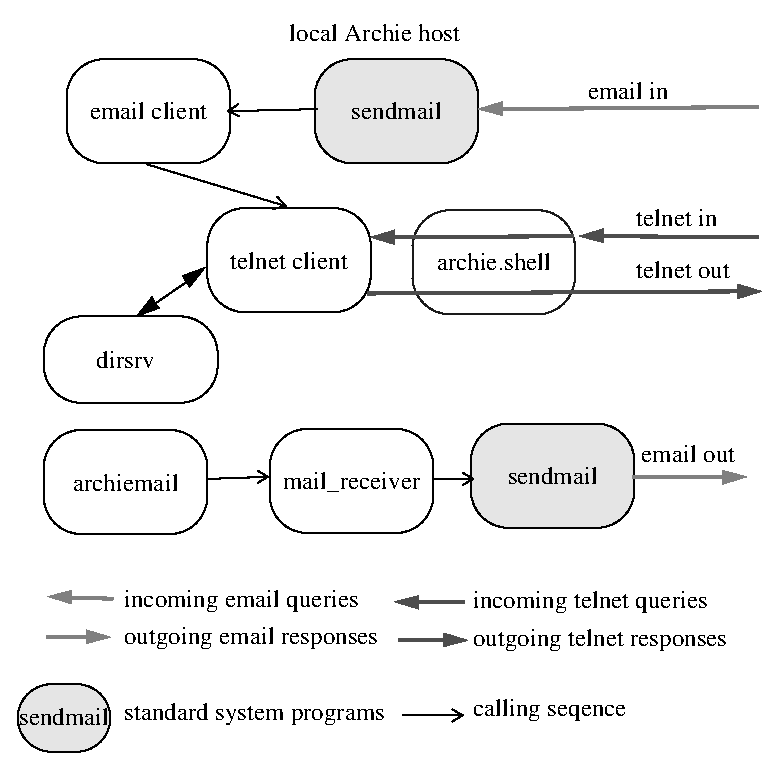
\epsfig{file=figs/telnet.eps,height=4in}
\end{center}
\caption{Archie system clients}
\label{fig:clients}
\end{figure}


\subsection{Client choices}

The telnet-client enables your user community to connect to an Archie server
and query the anonftp catalog through a standard telnet (remote login)
session. A user shell is provided and supports a query language to enable the
user to query the server. The email-client program enables users to send
electronic mail containing a series of commands to the Archie server which
will then be processed and returned in email to the user. You will have to
decide, as system administrator which of the supplied clients, if any you plan
to install. You should factor such things as

\begin{itemize}
\item Possible load on the system

\item Usefulness of the clients to your community

\item Administrative overhead
\end{itemize}


into your decision. The email and telnet clients can be run ``independently''
of one another in that you do not have to enable either one for the other one
to be made accessible.

\subsection{The  user system programs}

The following table describes the programs in the Archie user query
system. These programs can be found in the \Path{\archie/bin} directory.

\begin{tabular}{|l|p{5in}|}\hline

Program Name & Description \\ \hline \hline

telnet-client &

User interface via the telnet or rlogin protocols. The only program that
performs queries. Called by email-client to process queries. \\ \hline

email-client &

The user interface which processes incoming network email queries. \\ \hline

cgi-client &
The WWW interface that can be attached to your Web server to perform
queries. This will described in more details in section~\ref{sec:cgiclient} \\ \hline 

archie.shell &
Bourne shell script wrapper around the telnet-client which restricts the
number of simultaneous user telnet Archie sessions. (Optional). \\ \hline

archiemail &

``Front end'' to the Archie outgoing mail system. Used by the telnet-client
``mail'' command. Only used if the ``mail'' command or email-client are going
to be enabled. \\ \hline

mail\_receiver &

Does most of the work in sending mail to the user (generated by the ``mail''
command or from the email-client): parsing headers, compressing, encoding,
splitting and calling sendmail to mail the resulting data \\ \hline

split\_file &

Used to break large amounts of output into smaller pieces (if necessary),
since some mailers are only capable of dealing with messages of limited size.
\\ \hline
\end{tabular}


\subsection{The telnet client}

If you would like your user community to have access to the Archie system via
the standard telnet or rlogin programs, you should install the telnet client.

\subsubsection{Client privileges and security}

The installation phase (as described in ``Installing the basic Archie system''
on page~\pageref{chap:install}) will, in most cases, install the telnet client to operate as a
setuid (root) program. With these privileges, the client can change the
current

directory to the Archie home directory and call the chroot(2) system call to
make this the root of its own directory tree. This has the advantage of
reducing any unforeseen security problems when users use rlogin or telnet to
connect to the Archie server.



Whether the chroot call is made or not in the telnet client, the GNU less
program shipped with the Archie system has been modified to prevent the
examination of external files or execution of external processes. The modified
version of the sources for this program can be found in \Path{\archie/contrib.}




\alertbox{
The telnet client will relinquish its root status after it has performed this
chroot(2) system call, or exit if anything unusual occurs during the steps
leading up to (and including) the return from root status.

The telnet client will function even if it is not given permission to run with
root privileges.

For security reasons, on those platforms in which it is supported Bunyip
strongly recommends you install the telnet client to operate with root
privileges.}





If the telnet-client program is installed suid root and is running on a
platform which supports the chroot(2) security feature, copies of the system
files \Path{/etc/resolv.conf}, \Path{/etc/services}
(unless you are using NIS) and
\Path{/etc/termcap} must be placed in the \Path{\archie/etc} directory. This is because the
use of the chroot(2) system call will leave the original files inaccessible to
the Archie clients.





\subsubsection{Enabling the telnet mail feature}
\label{sec:telnetmail}

Most of the work of setting up the Archie client programs is done by the
installation script. However, you must first set up your system to accommodate
the new programs. This can be done as follows:

\begin{itemize}
\item
Create an archiemail entry in the /etc/services file (or the services
database, if you are running NIS) and in the \Path{/etc/services} file. For
example:

\param{archiemail 2709/tcp \#The Archie mail server}

\item
Create a corresponding entry in the /etc/inetd.conf file. For example:

\param{archiemail stream tcp nowait archie \Archie/bin/archiemail}

Don't forget to restart the inetd program (through the use of the UNIX kill
command, as described in ``The arserver program''on page~\pageref{sec:arserver}).


\item Create an alias, archie-errors, in the /etc/aliases file. This is where
errors generated by incorrect user mail addresses are sent, and is also the
Reply-To address in the mail responses sent to the user. To avoid dealing with
spurious email, you can set the alias to throw away incoming mail, by setting
the /etc/aliases entry to:

\param{archie-errors:/dev/null}

Remember to run, after these changes, the newaliases program or its NIS
equivalent (if you are using that system).

\item
Modify your sendmail configuration file. This is usually called sendmail.cf
and resides either in the \Path{/etc} or \Path{/usr/lib} directories. The
change that has to be made is to the T configuration lines. The default file
will look something like:



\param{\# Trusted users}

\param{Troot}

\param{Tdaemon} 

\param{Tuucp}

\noindent Now add the line:

\param{Tarchie}

This allows the Archie system to send mail with a ``Sender:'' of archie-errors
address. If this is not done, incorrectly addressed mail will bounce from the
remote mail receiver back to the Archie user, creating a mail loop which can
quickly fill your postmaster's mailbox.

After making this change you may need to ``compile'' your sendmail.cf file if
that is how your system is configured. Check to see if there is a file called
sendmail.fc in the same directory as the sendmail.cf file. If there is, the
run the following command:



\comm{sendmail -bz}


This will cause the sendmail configuration to be ``compiled'' (or ``frozen'').

\item
Modify the \Path{/etc/passwd} file for the archie user, with the full path for the
telnet-client program as the shell. For example:

\param{archie::23:1000:Archie User:<archie home>:<archie home>/bin/telnet-client}
\end{itemize}

\alertbox{
Note that, in this example, there is no password for the user archie. This is
normal for the operation of the most Archie installations. However, while you
are testing the system, you may wish to have a temporary password for this
account.}


Finally, check over the ``configure'' sections in the archiemail and
mail\_receiver scripts which reside in \Path{\archie/bin}. You should ensure that the
\Param{PATH} variable is correctly set to find the programs used by these
scripts. 



\subsubsection{Limiting the number of telnet sessions}
\label{sec:limit}

archie.shell is a shell script to limit the number of simultaneous connections
to the telnet-client.

\begin{itemize}
\item
Edit the archie.shell file to reflect the maximum number of simultaneous
sessions you want to allow, and the niceness level (see the UNIX manual entry
for nice(1)). The lines to be modified are clearly marked in the archie.shell
shell script.

\item
Edit the /etc/passwd file to change the archie user's shell from
telnet-client to archie.shell.

\item
A soft link between the telnet-client in \Path{\archie/bin} and -telnet-client
should exist from the default distribution. If it does not, run the following
command in that directory.

\comm{ln -s telnet-client -telnet-client}

\end{itemize}

\subsubsection{The .archierc file}

On start-up the telnet-client program reads a file called \Path{\archie/.archierc} if
it exists. The purpose of this file is to configure the program's behavior to
your particular needs. A number of variables can be set and commands executed
before the user prompt is generated. See the manual page archie\_clients(n) for
a complete explanation.

\subsubsection{Testing the telnet client}

Once the telnet-client program has been installed and configured, test it out
by performing a telnet session to the Archie host, and log in as
archie. Perform a ``find'' command to determine if everything is working
correctly.



\begin{itemize}
\item
The telnet client will not start on login:
\begin{itemize}
\item
Make sure the permissions on the file \Path{\archie/bin/telnet-client} are
correct. It should be executable by all, owned by root and run suid. That is
the ls(1) listing should look something like:

\param{---s--x--x 2 root 516096 Jul 16 02:22 telnet-client}
\end{itemize}


\item
The error message ``Can't resolve hostname (ardp)'' is displayed:

\begin{itemize}
\item
Check the telnet-client ``server'' variable (issue the command ``show
server''). It should be the valid name or IP address of an Archie host or in
many cases the name localhost if the telnet client and the dirsrv are running
on the same host.
\end{itemize}

\item
On start-up or after a command is issued an error is generated which says
``Timed out (ardp)'':

\begin{itemize}
\item
Check the telnet-client ``server'' variable (issue the command ``show
server''). It should be the valid name or IP address of an Archie host or in
many cases the name localhost if the telnet client and the dirsrv are running
on the same host.

\item
Make sure that the dirsrv process is running

\item
Check that the anonftp database has been initialized

\item
If using a remote (not local) Archie server host, it is possible that
network delays can cause this problem.
\end{itemize}
\end{itemize}


\subsection{The email client}
The email-client program allows users to access the Archie system via standard
Internet mail. It is in fact, just a specialized wrapper around the
telnet-client program which does the work of processing the incoming queries
(see Figure~\ref{fig:clients}). The requests from the email client are given
the lowest priority when queued on the Prospero server so as not to adversely
affect the operation of interactive clients.


The email-client can be used in one to two main ways, either ``interactively''
in which incoming email is processed as it is received, or ``batched'' in which
the incoming email is stored and processed later, usually at off-peak
times. In either case, to enable the email-client, first you need to enable
the telnet-client mail feature as described in section ``Enabling the telnet
mail feature'' on page~\pageref{sec:telnetmail}.

\subsubsection{``Interactive'' email requests}

For interactive email service add the following line to the /etc/aliases file.


\param{archie: ``| \Archie/bin/email-client''}



As usual, the newaliases program (or the NIS equivalent) will have to be run
in order for this change to take effect.

There are a number of options which can be provided to the email-client binary
including some to log incoming messages. See the archie\_clients manual page
for further details.



If your telnet-client binary is not installed as \Path{\archie/bin/telnet-client}
then you should use the ``-T'' option to tell the email client where the
telnet-client can be located.



\subsubsection{Batching email requests}
\label{sec:batch}

Email requests need not be processed directly as they are received on your
system. Instead, they can be batched and processed at a later (off-peak)
time. To do this change the standard entry in the /etc/aliases file to the
following:



\param{archie ``| <archie home>/bin/batch-email''}



By default, this will put each piece of mail in a separate file in
\Path{\archie/db/tmp}. You can override the temporary directory by using the -t
option to batch-email which will cause the email messages to be stored in an
alternate directory. You should make sure that this is a ``safe'' directory
whose contents will not be lost for example, on a system reboot.

You can then set your system to process the mail at a later time with the
process-email program.

\noindent For example, if you enter the line:



\param{0 1 * * * <archie home>/process-email}



into the crontab for archuser then each day at 01:00, the mail will be
processed. This also takes a -t option like batch-email to provide a different
temporary directory. process-email will process each piece of mail in
sequence.

\subsubsection{Testing the email client}

Test the email client by sending mail to \Param{archie@<your host name>}.  If
running as ``interactive'' email, a response should be generated in a number
of minutes. Note that this must be done from a machine other than the Archie
host due to the fact that on most systems, the sendmail program runs the user
daemon when mail is sent from off the local host, but as the user sending the
mail when run on the local host.



\alertbox{Email to the Archie server will not work from the Archie server host.}


\subsection{Auxiliary files}

The following files in \Path{\archie/etc} are used by the telnet-client and
email-client programs. They may be modified to reflect the local
configuration.


\begin{tabular}{|l|c|c|p{3.5in}|}\hline

Filename & \multicolumn{2}{c|}{Used By} & Description \\ \cline{2-3}
& telnet client & email client & \\ \hline \hline 

email.help & & x &
Response to a ``help'' command or an empty message. For any other form of more
specific help (e.g., ``help set''), the email-client returns the same
information provided by the telnet client. \\ \hline

manpage.ascii & x & x &
The pre-formatted version of the Archie manual page. \\ \hline

manpage.roff & x & x &
The troff(1) (or nroff(1)) version of the Archie manual page. \\ \hline

motd & x & x &
The ``message of the day'' that the email and telnet clients display to users at
the top of email messages or when they log in if set in dirsrv (See ``The
Message of the Day'' on page 52). \\ \hline

serverlist & x & x &
The list of servers given to the user in the ``servers'' command. \\ \hline

whatis & x & x &
The Archie whatis database. Entries (one per line) of short descriptions of
resources available on the network.
\\ \hline
\end{tabular}


\subsection{The Help system}
The Archie telnet and email client help system is rooted in the directory
\Path{\archie/help}. The system currently has full multi-lingual support. In order to
support languages other than the default supplied with the distribution, one
only need create a directory under \Path{\archie/help} with the name of that
language. For example a directory called francais would enable French language
support by allowing the users to type:



\param{archie> set help francais}



at the prompt in the telnet client or in the message body to the email
client. The files in the \Path{\archie/help/english} need then to be translated into
the new language. The files containing the actual data are called `=' and the
subdirectory names themselves provide the menu for that part of the help
system. See the manual page archie\_clients(n) for further details.


\subsection{Quoting in the clients}

For the email and telnet Archie clients, quoting in the command-line
interpreter is handled in much the same way as for the standard csh (see the
man page csh(1)). So, for example, the `.' can be treated as follows:



\param{LIST .il}

The `.' is treated as a regular expression

\param{LIST \\.il}

The `.' is quoted, and passed along (untouched) to the Archie search also if
you specify

\param{LIST il\$}

you will make sure that the host names returned end with the string ``il''.
For further details on regular expression consult the regexp(3) manual.





\section{Webindex catalog clients} 


This section takes a brief look at the WWW client. It provides access to both
webindex and anonftp catalogs.  Note that this section is still under
construction and any comment is very much welcomed. \new


\subsection{The cgi-client}
\label{sec:cgiclient}

The files are:

\begin{tabular}{ll}

cgi/html/archie.html      & Simple search form \\

cgi/html/archie-adv.html  & Advanced search form \\

cgi/html/archie-help.html & Help page \\

cgi/bin/archie.cgi & perl script called by the HTML forms \\ 

cgi/bin/cgi-client & binary called by the perl script \\

\end{tabular}



\subsubsection{Where to put them ?}

In order to provide a consistent way for accessing the Archie database,
we think that the urls should always be of the same format for
all public Archie server.

This format being

\path{http://archie.foo.bar/archie.html}

\path{http://archie.foo.bar/archie-adv.html}

\path{http://archie.foo.bar/archie-help.html}

We need to specify the \Path{.html} extension to ensure that all
WWW server will actually return the documents as  HTML documents. Otherwise,
some will presume that they are simply ascii.

\subsubsection{Configuration}

The configuration procedure is as follows:

\begin{enumerate}

\item Move the .html and .gif files to where your web pages are accessed.
\item Move (or link) ``archie.cgi'' to the cgi-bin directory of your web server.
\item
Edit the html files ``archie.html'' and ``archie-adv.html'' to reflect
the appropriate path of the cgi script ``archie.cgi'' after you have placed
it in the right path.

\item 
Edit the file ``archie.cgi'' and configure the first few lines as indicated
in the file.

\item Make sure that the UID for the ``cgi-client'' binary is set.


\item
Test the forms and if you don't like the format of the output, take a
look at the ``archie.cgi'' perl script and edit the output variables to your
convenience.
\end{enumerate}


\subsubsection{How does it work}

The ``archie.cgi'' perl script receives a query (from the archie*.html forms)
and calls up ``cgi-client''. The cgi-client binary processes the request and
sends the results to the perl script in plain record-template format.
``archie.cgi'' reads the results, reformats the output into HTML and then
sends the new output to the web server.



\subsubsection{How to reformat the output}

``archie.cgi'' is the perl script you need to modify.  The second segment
after the configuration part holds the variables that are sent back to the
Web server.  Configure any variable to your needs.
  

\subsubsection{Where is the information logged}

``cgi-client'' logs queries, the number of hits and any error messages to a
file in the log file \Path{\archie/logs/query.log}



